% !TeX program = pdflatex
\documentclass[preprint,12pt]{elsarticle}
\journal{Computer Networks}
\usepackage{amsmath,amssymb,amsthm,booktabs,graphicx,algorithm,algorithmic,multirow}
\usepackage{float}
\newtheorem{proposition}{Proposition}
\emergencystretch=1.5em
\usepackage{tikz}
\usetikzlibrary{arrows.meta,positioning,fit,calc}

\begin{document}
\begin{frontmatter}
\title{FedRAS: Network-Conditioned Rank Allocation for Federated LoRA}
\author[inst1,inst2,inst3]{Wenyu Ma}
\author[inst1,inst2,inst3]{Tao Hu\corref{cor1}}
\ead{hutaondsc@163.com}
\author[inst1,inst2,inst3]{Xinlei Liu}
\cortext[cor1]{Corresponding author}
\address[inst1]{Information Engineering University, Zhengzhou 450001, China}
\address[inst2]{Key Laboratory of Cyberspace Endogenous Safety and Security of Henan Province, Zhengzhou 450001, China}
\address[inst3]{Key Laboratory of Cyberspace Security, Ministry of Education of China, Zhengzhou 450001, China}

\begin{abstract}
In mobile-edge federated learning, uplink links are time-varying and deadline-bound, and full-parameter updates frequently miss their deadlines when links degrade. Federated LoRA reduces the payload, but existing systems treat the rank as a training hyperparameter, ignoring the coupling that the rank itself determines the payload and the payload determines the delivery probability: a larger rank buys adaptation capacity but is more likely to miss the deadline. We formalize rank selection and client admission as a joint scheduling problem under deadline constraints and propose FedRAS, which scores every client--rank pair with a payload-conditioned delivery risk and a saturating capacity gain, solves the assignment exactly with a dynamic program under a byte budget and a participation cap, and aggregates heterogeneous ranks with frozen-factor rank masking. The design comes with mechanism-level guarantees: the grid assignment is exact on the stated budget grid, the budget regime in which a per-client greedy rule is already optimal is characterized in closed form, and frozen-factor aggregation of heterogeneous ranks is exact. The gains come from delivering more updates within the deadline rather than from changing training, which is why accuracy remains statistically equivalent while the network-side outcomes improve. On a real trainer, FedRAS delivers 22\% more timely updates with 23\% fewer bytes than fixed rank 16 under deadline stress at statistically equivalent accuracy, while full-parameter updates miss every stress deadline; link-oblivious low-rank schedules trade adaptation capacity for delivery, and FedRAS holds the high-capacity end of that trade-off; and, at 500 clients, exact scheduling beats greedy heuristics whenever the budget binds, at sub-second per-round cost.
\end{abstract}

\begin{keyword}
Federated LoRA \sep Mobile edge computing \sep Rank selection \sep Deadline scheduling \sep Wireless federated learning
\end{keyword}
\end{frontmatter}

\section{Introduction}
\label{sec:intro}

Mobile edge networks increasingly host federated learning (FL) workloads, with clients that include smartphones, vehicles, UAV terminals, and satellite-connected devices \cite{mcmahan2017fedavg,kairouz2021advances,nguyen2021iotfl,liu2018sagin,mahboob2024ntn}. The dominant cost of such systems is the uplink: full-parameter model updates saturate wireless capacity, drain client energy, and frequently miss round deadlines when links degrade during handover or outage \cite{hamdi2022ehfl,razmi2022ground,tang2023flsagin,qin2024dfrl,ribero2023intermittent}. Low-rank adaptation (LoRA) has therefore become an attractive transmission format, because each adapted layer communicates only two small factor matrices instead of the full weight delta \cite{hu2022lora,babakniya2023slora,zhang2024fedit}.

Existing federated LoRA systems, however, treat the rank $r$ as a model hyperparameter, whether fixed across the fleet \cite{sun2024ffalora,zhang2023fedpetuning}, varied across clients \cite{cho2024hetlora,fan2025helora}, adapted across rounds \cite{wu2026fedara,yang2024safedlora}, or personalized through model-heterogeneous and dual-adapter designs \cite{yi2026pfedlora,yang2024feddpa}. In all of these systems the rank is selected from data and system constraints alone, never from the state of a lossy, deadline-constrained link. This convention ignores a scheduling dimension that is directly visible to the network. The omitted coupling is mechanical: a larger rank transmits more bytes and therefore loses delivery probability exactly where it gains adaptation capacity, while a smaller rank travels light but forfeits capacity on the healthy links that could have carried it. Whether the extra capacity is worth the delivery risk depends on the link state, and no training-side rule observes that state. Each round must therefore decide jointly, under a byte budget and a participation cap, which clients participate and at what rank.

This raises three questions that must be answered. First, how should the delivery probability depend on the rank and the observable link state? The rank directly determines the payload size, and the payload determines whether an update can meet the deadline on a lossy link, so the delivery model must take the rank as an argument rather than an afterthought. Second, how should the client--rank assignment be solved under budget and participation constraints? The problem is a multiple-choice knapsack with an admission constraint, greedy rules are not necessarily optimal, and one must establish when exact solving is necessary and when it may degrade to a cheap rule. Third, does the resulting adaptation improve network behavior in a real trainer? The scheduling objective is a network-side utility, not the training accuracy, and the two need not agree, so the validation must show that accuracy does not degrade because of the scheduling.

We answer these questions with a delivery model, a grid-based dynamic-programming solver, a rank-selection rule, and a two-tier evaluation, and call the resulting method FedRAS. Our contributions are threefold.

\begin{itemize}
\item \textbf{FedRAS framework.} We propose FedRAS, to our knowledge the first framework that treats the LoRA rank as a deadline-constrained, network-conditioned, schedulable resource: each round, client admission and rank are decided jointly under a byte budget and a participation cap, with payloads accounted at their real serialized sizes (Section~\ref{sec:model}).
\item \textbf{Theoretical analysis.} We prove exactness of the grid assignment (Proposition~\ref{prop:dp}), the budget-feasibility condition under which the cheap per-client rule is already optimal (Proposition~\ref{prop:cohort}), and exact frozen-factor aggregation of heterogeneous ranks (Proposition~\ref{prop:agg}), with bounded time and memory cost (Section~\ref{sec:theory}).
\item \textbf{Experiments and validation.} On a real federated LoRA trainer and a 500-client scheduler simulation, FedRAS delivers 22\% more timely updates with 23\% fewer bytes than fixed rank 16 under deadline stress at statistically equivalent accuracy, while full-model updates miss every stress deadline; the conclusions are robust across datasets, link profiles, and delivery-predictor distortions (Section~\ref{sec:eval}). Accuracy, timely delivery, and bytes are reported as separate outcomes throughout.
\end{itemize}

A preliminary poster version of this work studied joint client--protection scheduling for federated learning in space--air--ground mobile networks \cite{ma2026mswim}. The present article substantially reformulates that line of work around a different schedulable resource. It replaces compression-and-protection policies with the LoRA rank as the per-client decision variable. It introduces the real-payload delivery hazard and the saturating capacity model of Section~\ref{sec:model}, replaces the heuristic admission-and-repair procedure with a dynamic program that is exact on the stated budget grid, and adds frozen-factor rank-masked aggregation for heterogeneous ranks. It also reports a new two-tier evaluation comprising a real federated LoRA trainer, a 500-client scheduling simulator, and a solver exactness study. Accordingly, all numerical results in this article come from the revised formulation and implementation and are not comparable with the preliminary version.

The remainder of this paper is organized as follows. Section~\ref{sec:related} reviews related work. Section~\ref{sec:model} presents the system model, the adversary and trust assumptions, and the scheduling formulation. Section~\ref{sec:solver} describes the FedRAS design and Section~\ref{sec:theory} its theoretical analysis. Section~\ref{sec:eval} reports the experimental evaluation, Section~\ref{sec:discussion} discusses interpretation, deployment, and limitations, and Section~\ref{sec:conclusion} concludes.

\section{Related work}
\label{sec:related}

\subsection{Federated LoRA and heterogeneous-rank adaptation}
\label{sec:rwlora}
LoRA freezes a pretrained backbone and learns low-rank increments $\Delta W=BA$ \cite{hu2022lora}. Federated LoRA trains these adapters across clients. Prior work has studied sparse updates and instruction tuning \cite{babakniya2023slora,zhang2024fedit}, examined how standard parameter-efficient tuning behaves under the federated setting \cite{zhang2023fedpetuning}, and pursued personalization through model-heterogeneous or dual-adapter designs \cite{yi2026pfedlora,yang2024feddpa}. A further line lets the rank vary across clients and aligns heterogeneous ranks for aggregation, by rank self-pruning with sparsity-weighted averaging \cite{cho2024hetlora}, stacking \cite{wang2024flora}, zero-padded rank alignment \cite{fan2025helora}, or SVD-based dynamic rank allocation \cite{wu2026fedara}.

FFA-LoRA \cite{sun2024ffalora} froze one factor at its random initialization and showed that this improves stability in privacy-preserving federated fine-tuning. We adopt the same frozen-factor property for a stronger reason. When the frozen factor is identical across clients, averaging the trainable factor gives exact coordinate-wise averaging of the active induced-update slices, as Proposition~\ref{prop:agg} shows, and each client uploads only that factor. It thereby removes the factor-rotation ambiguity that makes joint factor averaging differ from update averaging. Section~\ref{sec:aggregation} develops this aggregation.

SA-FedLoRA schedules rank over rounds without conditioning on link state \cite{yang2024safedlora}. FedSA-LoRA studies asymmetric factor aggregation with client-local parameters \cite{guo2025fedsalora}. Across these systems, the rank responds to training progress, parameter importance, or device capability; in none of them is it a decision variable conditioned on the delivery state of a deadline-constrained link. We evaluate an annealing baseline and joint A/B averaging while making rank a per-round decision conditioned on delivery state and deadline.

\subsection{Communication-efficient federated learning}
A broad literature reduces FL communication through sparsification, quantization, compressed sensing, and over-the-air aggregation \cite{oh2023fedqcs,oh2024fedvqcs,liu2023adaptivequant,kim2023beamforming,reisizadeh2020fedpaq,lin2018deep}. These methods compress a given update. Our scheduler selects its rank before transmission, so rank directly affects payload and deadline feasibility. The proposed capacity and delivery models can therefore be combined with other codecs.

\subsection{Client selection and deadline-aware scheduling}
\label{sec:rwselect}
Client selection improves FL efficiency under data, latency, and energy heterogeneity. Oort ranks candidates by a utility that couples data value with system efficiency \cite{oort2021oort}; FedCS selects clients under explicit resource constraints \cite{nishio2019fedcs}; TiFL groups clients into latency tiers to bound stragglers \cite{chai2020tifl}; further designs target cost and freshness \cite{chen2024clientselection,dong2024aoi,luo2021costeffective}. A second line makes network scheduling deadline- and reliability-aware in mobile and non-terrestrial networks, from client participation \cite{razmi2022ground,tang2023flsagin,ribero2023intermittent,han2024orchestrating} to traffic offloading driven by federated reinforcement learning \cite{qin2024dfrl}: LESSON admits wireless clients at differentiated frequencies under a latency budget \cite{yu2023lesson}, and FedSN coordinates federated training across heterogeneous LEO satellite networks \cite{lin2025fedsn}. These methods generally treat update size as fixed: participation is decided for a given payload, not jointly with it. We include an Oort-style selector as a selection baseline. FedRAS chooses participation and update rank together, yielding a multiple-choice knapsack.

\subsection{Research gap and positioning}
Across these lines, a common interface is missing. The rank-adaptation methods of Section~\ref{sec:rwlora} decide the rank from training state, parameter importance, or device capability; the selection and deadline-aware methods of Section~\ref{sec:rwselect} decide participation for a fixed update size. Neither treats the LoRA rank as a schedulable network resource whose payload sets the delivery probability on a lossy link, and none formulates the joint client--rank assignment under byte-budget and deadline constraints. Table~\ref{tab:rwcompare} positions FedRAS against the closest systems along these dimensions.

We do not claim each ingredient individually as new. Our contribution is their combination: the LoRA rank treated as a deadline-constrained network resource with an explicit payload-conditioned delivery hazard, a client--rank assignment that is exact on the stated budget grid with quantified greedy gaps and solver cost, and validation with a real federated trainer in which adapters are placed on every block of the backbone and all byte accounting uses real serialized sizes. The theoretical contribution is mechanism correctness rather than a learning-performance guarantee: exactness of the assignment on the stated grid (Proposition~\ref{prop:dp}) and exactness of frozen-factor aggregation (Proposition~\ref{prop:agg}), each with its scope conditions stated where it applies. The claim is conditional on the surveyed literature of Section~\ref{sec:related} and on the evaluated setting.

\begin{table}[t]
\centering
\caption{Positioning against federated LoRA and client-selection systems. \checkmark{} = the property holds in the cited papers' own descriptions; $\times$ = absent or not reported. Delivery-aware means that a scheduling or adaptation decision conditions on per-round network delivery state (rate, deadline, delivery probability) rather than on training progress, device capability, or static profiling alone. Real payload means payload is accounted as transmitted bytes rather than a fixed or parameter-count proxy. Real training means model training is executed in the evaluation as reported.}
\label{tab:rwcompare}
\footnotesize
\setlength{\tabcolsep}{4pt}
\renewcommand{\arraystretch}{1.05}
\begin{tabular}{l ccccccc}
\toprule
System & \shortstack[r]{Var.\\rank} & \shortstack[r]{Deliv.-\\aware} & \shortstack[r]{Het.-rank\\agg.} & \shortstack[r]{Admis-\\sion} & \shortstack[r]{Joint\\adm.+rank} & \shortstack[r]{Real\\payload} & \shortstack[r]{Real\\training}\\
\midrule
FFA-LoRA \cite{sun2024ffalora} & $\times$ & $\times$ & $\times$ & $\times$ & $\times$ & $\times$ & \checkmark\\
SLoRA \cite{babakniya2023slora} & $\times$ & $\times$ & $\times$ & $\times$ & $\times$ & $\times$ & \checkmark\\
FedDPA \cite{yang2024feddpa} & $\times$ & $\times$ & $\times$ & $\times$ & $\times$ & $\times$ & \checkmark\\
HetLoRA \cite{cho2024hetlora} & \checkmark & $\times$ & \checkmark & $\times$ & $\times$ & $\times$ & \checkmark\\
HeLoRA \cite{fan2025helora} & \checkmark & $\times$ & \checkmark & $\times$ & $\times$ & $\times$ & \checkmark\\
FedARA \cite{wu2026fedara} & \checkmark & $\times$ & \checkmark & $\times$ & $\times$ & $\times$ & \checkmark\\
SA-FedLoRA \cite{yang2024safedlora} & \checkmark & $\times$ & $\times$ & $\times$ & $\times$ & $\times$ & $\times$\\
FedSA-LoRA \cite{guo2025fedsalora} & $\times$ & $\times$ & $\times$ & $\times$ & $\times$ & $\times$ & \checkmark\\
\midrule
Oort \cite{oort2021oort} & $\times$ & $\times$ & $\times$ & \checkmark & $\times$ & $\times$ & \checkmark\\
FedCS \cite{nishio2019fedcs} & $\times$ & \checkmark & $\times$ & \checkmark & $\times$ & $\times$ & \checkmark\\
TiFL \cite{chai2020tifl} & $\times$ & $\times$ & $\times$ & \checkmark & $\times$ & $\times$ & \checkmark\\
LESSON \cite{yu2023lesson} & $\times$ & \checkmark & $\times$ & \checkmark & $\times$ & $\times$ & \checkmark\\
FedSN \cite{lin2025fedsn} & $\times$ & \checkmark & $\times$ & \checkmark & $\times$ & $\times$ & \checkmark\\
\midrule
\textbf{FedRAS (ours)} & \checkmark & \checkmark & \checkmark & \checkmark & \checkmark & \checkmark & \checkmark\\
\bottomrule
\end{tabular}
\end{table}

\section{System model and threat model}
\label{sec:model}

\begin{figure}[t]
\centering
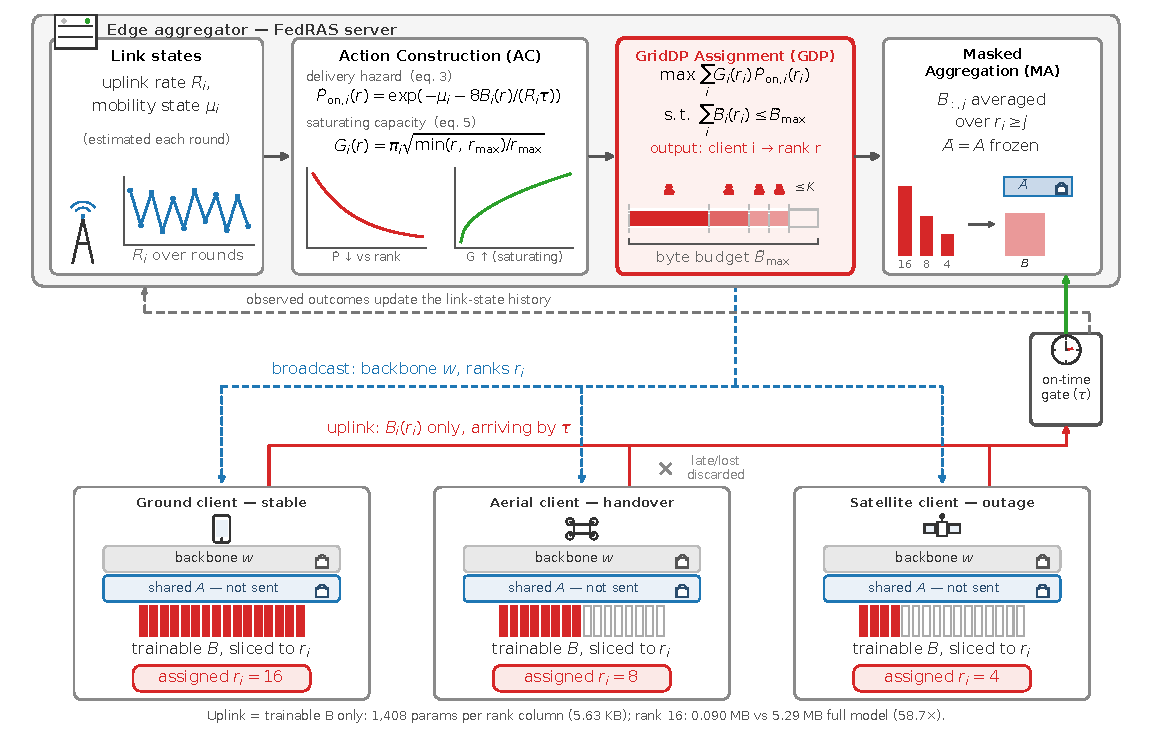
\includegraphics[width=0.98\columnwidth]{recolored_figures/fig_architecture}
\caption{FedRAS round pipeline. Action Construction (AC) scores every client--rank pair with the delivery hazard \eqref{eq:hazard} and the saturating capacity \eqref{eq:cap}; the GridDP assignment (GDP) computes the client--rank assignment under the byte budget and the admission cap. Updates arriving within the deadline $\tau$ pass the on-time gate and are merged by Masked Aggregation (MA) while the shared factor $A$ stays frozen; observed outcomes update the link-state history. AC, GDP, and MA correspond to Algorithms~\ref{alg:ac}--\ref{alg:ma}; the overall round is Algorithm~\ref{alg:fedras}.}
\label{fig:architecture}
\end{figure}

\subsection{Mobile-edge federated learning architecture and round protocol}
We consider a mobile edge network in which an edge aggregator serves a client set
$\mathcal{D}=\mathcal{D}_g\cup\mathcal{D}_a\cup\mathcal{D}_s$ of ground clients $\mathcal{D}_g$, aerial and UAV clients $\mathcal{D}_a$, and satellite-connected clients $\mathcal{D}_s$. Ground links are comparatively stable, aerial links face frequent handover, and satellite links suffer long propagation delay, intermittent visibility, and outages \cite{mahboob2024ntn,razmi2022ground}. The aggregator holds the global model, schedules every round, and aggregates the timely updates.

Let $w^t$ denote the frozen backbone broadcast at round $t$. Client $i$ trains LoRA factors $A_{i,\ell}$ and $B_{i,\ell}$ for the adapted layers $\ell\in\mathcal L$, with effective weight change $\Delta W_{i,\ell}=B_{i,\ell}A_{i,\ell}$. A rank $r$ update uses the first $r$ columns of $B_{i,\ell}$ and the matching rows of the shared $A$. Fig.~\ref{fig:architecture} shows the resulting round pipeline. In every round, the aggregator estimates the link states, scores the client--rank actions with Action Construction (AC, Section~\ref{sec:ac}), and solves the assignment with the GridDP assignment (GDP, Section~\ref{sec:gdp}); the admitted clients train locally with their factors sliced to the assigned rank, so only the first $r$ coordinates receive gradient updates, and upload before the deadline $\tau$; the aggregator then merges the timely updates with Masked Aggregation (MA, Section~\ref{sec:aggregation}) and updates its link-state history from the observed outcomes. Late or lost updates are discarded, because stale updates harm convergence stability in deadline-critical federated learning. The experiments evaluate both a homogeneous link profile and a grouped ground--aerial--satellite profile with distinct rate and mobility laws (Section~\ref{sec:eval}).

\subsection{Link, mobility, and timely-delivery model}
At decision time the scheduler receives an estimated uplink rate $\bar R_i^t$ in Mbps and a mobility state. The realized rate $R_i^t$, handover event $H_i^t\in\{0,1\}$, and packet loss indicator $J_i^t$ are not observed before transmission. For an update of $B_i^t(r)$ megabytes, the modeled delivery time is
\begin{equation}
T_i^t(r)=T_{\rm train,i}(r)+T_{\rm proc,i}(r)+\frac{8B_i^t(r)}{R_i^t}+d_i^t+H_i^t\Delta d_h.
\label{eq:delivery}
\end{equation}
Timely delivery is the event
\begin{equation}
P_{\rm on,i}^t(r)=\Pr\!\left(T_i^t(r)\le\tau,\;J_i^t=0\mid x_i^t\right).
\label{eq:pon}
\end{equation}

The implementation uses the following hazard surrogate rather than a derived distribution for all terms in \eqref{eq:delivery}.
\begin{equation}
\hat P_{\rm on,i}^t(r)=\exp\!\big(-\mu_i^t\big)\exp\!\Big(-\frac{8B_i^t(r)}{\bar R_i^t\tau}\Big).
\label{eq:hazard}
\end{equation}
The dimensionless intensity $\mu_i^t$ summarizes mobility-related failure risk, packet loss, handover effects, and unmodeled processing time; it is a fixed surrogate rather than an estimated distribution in the present implementation, and \eqref{eq:hazard} is used as a plug-in predictor throughout. The construction of the estimated states and the sensitivity studies are specified in Section~\ref{sec:eval}; how far the conclusions survive this idealization is delimited in Section~\ref{sec:discussion}.

\subsection{Rank-dependent payload and adaptation capacity}
With $b$ bits per parameter and the frozen factor $A$ shared and never transmitted, a rank-$r$ client uploads only the trainable factor $B$, whose per-rank cost is the summed output dimension $D=\sum_{\ell\in\mathcal L}d_\ell$ of the adapted layers. The real serialized payload is
\begin{equation}
B_i^t(r)=\frac{b}{8}\,r\,D+B_{\rm meta},
\label{eq:size}
\end{equation}
in bytes. Rank is therefore a network-visible resource: it scales both the adaptation capacity and the transmission time, and its per-unit payload is audited against the evaluated model in Section~\ref{sec:eval}. We model the useful contribution of a delivered rank-$r$ update with the saturating capacity gain
\begin{equation}
G_i^t(r)=\pi_i^t\,\sqrt{\min(r,r_{\max})/r_{\max}},
\label{eq:cap}
\end{equation}
where $\pi_i^t$ is a per-client contribution prior in the spirit of Oort-style utility \cite{oort2021oort}. The width $r_{\max}$ is the factor width provisioned at all clients. The square root encodes the diminishing returns of rank that the delivered-update norms exhibit directly in the trainer (Section~\ref{sec:traineval}), and the saturation at $r_{\max}$ reflects that wider factors add payload but no expressible capacity once the provisioned width is reached. Full-parameter FedAvg updates are accounted at their true serialized size (Table~\ref{tab:audit}).

\subsection{Adversary and trust model}
Clients are honest but curious: they follow the training protocol, and raw data never leaves the devices, which is the standing premise of federated learning on this infrastructure. The edge aggregator is trusted scheduling infrastructure: it observes link states, client--rank assignments, and delivered update factors, and runs the aggregation of Section~\ref{sec:aggregation}. The external adversary of interest is an eavesdropper on the wireless uplink who observes the transmitted $B$ factors. Because the frozen factor $A$ is public and a rank-$r$ client transmits only its first $r$ coordinates, the object reconstructable from an intercepted transmission is the rank-$r$ induced update, and the exposed surface is its $B$-slice: a transmission strictly smaller in bytes and in exposed coordinate count than a joint-factor or full-model update. This is a reduction in exposed transmission, not a protection mechanism; FedRAS proposes none, and differential-privacy accounting, secure aggregation, and Byzantine robustness are orthogonal and out of scope (Section~\ref{sec:discussion}).

\subsection{Deadline-constrained client--rank scheduling formulation}
\label{sec:problem}

Each round, the aggregator decides $a_i^t\in\{0\}\cup\mathcal R$, where $a_i^t=0$ means client $i$ does not participate and $a_i^t=r$ schedules it at rank $r$. The per-round problem is
\begin{equation}
\max_{\{a_i^t\}}\;\sum_{i\in\mathcal D}\mathbf 1\{a_i^t>0\}\,G_i^t(a_i^t)\,P_{\rm on,i}^t(a_i^t)
\label{eq:objective}
\end{equation}
\begin{equation}
\text{s.t.}\quad \sum_i B_i^t(a_i^t)\le B_{\max},\qquad \sum_i\mathbf 1\{a_i^t>0\}\le K .
\label{eq:constraints}
\end{equation}
The objective is a scheduling utility: expected useful delivered updates under the byte budget $B_{\max}$ and the participation cap $K$. It is a network-side objective, not a surrogate for final test accuracy; increasing $r$ raises $G$ sublinearly while raising payload and lowering the delivery surrogate. The experiments therefore report test accuracy, timely delivery ratio, bytes per round, and mean delivered rank as separate outcomes (Section~\ref{sec:eval}).

\section{FedRAS design}
\label{sec:solver}

\subsection{Overview}
Algorithm~\ref{alg:fedras} summarizes one scheduling round as a fixed sequence of three named components. Action Construction (AC, Section~\ref{sec:ac}) scores every client--rank pair with a real payload, a delivery probability, and a capacity gain; the GridDP assignment (GDP, Section~\ref{sec:gdp}) solves the scored assignment exactly under the byte budget and the admission cap, with a cheap per-client rule covering the unconstrained regime; and Masked Aggregation (MA, Section~\ref{sec:aggregation}) merges heterogeneous-rank updates toward the frozen shared factor. Fig.~\ref{fig:architecture} places AC, GDP, and MA in the round pipeline. The design contains no training-side logic: admissions and ranks are chosen from network state alone.

\begin{algorithm}[t]
\caption{FedRAS Round}
\label{alg:fedras}
\begin{algorithmic}[1]
\REQUIRE clients $\mathcal D$, rank set $\mathcal R$, cap $K$, budget $B_{\max}$, deadline $\tau$, link-state history $\mathcal H^{t-1}$
\ENSURE assignment $a^t$; new adapter state $S^t$; updated history $\mathcal H^t$
\STATE estimate per-client link states $x_i^t$ from $\mathcal H^{t-1}$
\STATE score all pairs $(i,r)$: utilities $u_i(r)$ and integer costs $\widetilde B_i(r)$ (AC, Algorithm~\ref{alg:ac})
\STATE solve the assignment $a^t$ under $K$ and $B_{\max}$ (GDP, Algorithm~\ref{alg:gdp}); when the all-$r_{\max}$ profile is budget-feasible, the per-client maximizer rule is already optimal (Proposition~\ref{prop:cohort})
\STATE broadcast the backbone $w^t$; admitted clients train locally with factors sliced to $a_i^t$ and upload before $\tau$
\STATE pass uploads arriving within $\tau$ (on-time gate)
\STATE aggregate timely updates with the frozen shared $A$ (MA, Algorithm~\ref{alg:ma})
\STATE append observed outcomes (timely, late, lost) to $\mathcal H^t$
\end{algorithmic}
\end{algorithm}

\subsection{Action Construction (AC)}
\label{sec:ac}
Each round the aggregator selects, for every client, one action from the discrete set $a_i^t\in\{0\}\cup\mathcal R$ of Section~\ref{sec:problem}. AC builds and scores this action set (Algorithm~\ref{alg:ac}): the per-rank payload follows \eqref{eq:size}, the delivery hazard \eqref{eq:hazard} and the capacity gain \eqref{eq:cap} give the estimated utility $u_i(r)=G_i^t(r)\hat P_{\rm on,i}^t(r)$, and a conservative ceiling discretization onto a budget grid $q$ yields the integer cost $\widetilde B_i(r)=\lceil B_i^t(r)/q\rceil$. The same grid is applied to the dynamic program, the greedy baselines, and the admission checks, so that every scheduling method optimizes over the identical feasible region. Under this discretization, the single-round estimated problem \eqref{eq:objective}--\eqref{eq:constraints} is a multiple-choice knapsack with an admission constraint, for which an exact pseudo-polynomial dynamic program exists; the evaluated grid width and its quantization error are quantified in Section~\ref{sec:dp_study}.

\begin{algorithm}[t]
\caption{Action Construction (AC)}
\label{alg:ac}
\begin{algorithmic}[1]
\REQUIRE clients $\mathcal D$, ranks $\mathcal R$, budget grid $q$, link states $\{x_i^t\}$
\ENSURE scored action set $\{u_i(r),\,\widetilde B_i(r)\}_{i\in\mathcal D,\,r\in\mathcal R}$
\FOR{each client $i$ and rank $r$}
  \STATE payload $B_i^t(r)$ by \eqref{eq:size}; integer cost $\widetilde B_i(r)\gets\lceil B_i^t(r)/q\rceil$
  \STATE delivery probability $\hat P_{\rm on,i}^t(r)$ by \eqref{eq:hazard}; capacity $G_i^t(r)$ by \eqref{eq:cap}
  \STATE utility $u_i(r)\gets G_i^t(r)\,\hat P_{\rm on,i}^t(r)$
\ENDFOR
\STATE return the scored set; pairs with $\widetilde B_i(r)>\widetilde B_{\max}$ are infeasible
\end{algorithmic}
\end{algorithm}

\subsection{GridDP Assignment (GDP)}
\label{sec:gdp}
GDP solves the scored assignment exactly (Algorithm~\ref{alg:gdp}). Let $V_i(k,b)$ be the maximum estimated utility from the first $i$ clients with $k$ admissions and integer budget $b$. Initialize $V_0(0,0)=0$ and all other states to $-\infty$. The recurrence is
\begin{equation}
V_i(k,b)=\max\Big\{V_{i-1}(k,b),\;\max_{r\in\mathcal R}\big[V_{i-1}(k-1,b-\widetilde B_i(r))+u_i(r)\big]\Big\},
\label{eq:dp}
\end{equation}
where $u_i(r)=G_i^t(r)\hat P_{\rm on,i}^t(r)$. Backpointers recover the assignment. Propositions~\ref{prop:dp} and~\ref{prop:cohort} (Section~\ref{sec:theory}) establish the exactness of this recurrence and the regime in which the per-client maximizer rule $r_i^\star$ is already optimal, in which case GDP reduces to that rule at zero cost.

\begin{algorithm}[t]
\caption{GridDP Assignment (GDP)}
\label{alg:gdp}
\begin{algorithmic}[1]
\REQUIRE scored actions $\{u_i(r),\,\widetilde B_i(r)\}$ from AC, cap $K$, budget grid $\widetilde B_{\max}$
\ENSURE client--rank assignment $a^t$
\STATE $V_0(0,0)\gets 0$; all other DP states $\gets -\infty$
\FOR{each client $i\in\mathcal D$}
  \FOR{$k=0,\dots,K$ and each budget state $b$}
    \STATE $V_i(k,b)\gets$ skip or best rank transition of \eqref{eq:dp}
    \STATE store the maximizing action as a backpointer
  \ENDFOR
\ENDFOR
\STATE backtrack from $\max_{k,b}V_{|\mathcal D|}(k,b)$; return $a^t$
\end{algorithmic}
\end{algorithm}

\subsection{Masked Aggregation (MA)}
\label{sec:aggregation}
Clients scheduled at different ranks share an $r_{\max}$ coordinate system. For one adapted layer, client $i$ has sample weight $n_i$ and delivered rank $r_i$. The factor $A\in\mathbb R^{r_{\max}\times k}$ is frozen and shared, while $B_i\in\mathbb R^{d\times r_{\max}}$ is trainable. A rank $r_i$ update activates columns $1$ through $r_i$ of $B_i$ and the matching rows of $A$, giving $\Delta W_i=\sum_{j\le r_i}[B_i]_{:,j}[A]_{j,:}$.

Jointly trained factor pairs $(A_i,B_i)$ are identifiable only up to invertible transforms, so separately averaged factors need not average the updates at all. The elevated-learning-rate ablation of Section~\ref{sec:eval} examines this aggregation rule empirically.

\textbf{Rank-masked averaging.} The server zero-pads inactive columns of each delivered $B_i$ and averages each active coordinate over the clients that activate it,
\begin{equation}
\bar B_{:,j}=\frac{1}{W_j}\sum_{i:\,r_i\ge j} n_i\,\big[B_i\big]_{:,j},
\qquad
W_j=\sum_{i:\,r_i\ge j} n_i ,
\label{eq:maskavg}
\end{equation}
while the frozen factor aggregates to itself, $\bar A=A$. The server then applies momentum per factor tensor. With $\Delta^t=\bar B-S^{t-1}$, the velocity and state update as $v^t=\beta\,v^{t-1}+(1-\beta)\,\Delta^t$ and $S^t=S^{t-1}+v^t$, with damping coefficient $\beta$ absorbing client-sampling and link noise. Algorithm~\ref{alg:ma} fixes the procedure; Proposition~\ref{prop:agg} (Section~\ref{sec:theory}) states its exactness and dilution properties.

\begin{algorithm}[t]
\caption{Masked Aggregation (MA)}
\label{alg:ma}
\begin{algorithmic}[1]
\REQUIRE timely updates $\{(n_i,B_i,r_i)\}$, frozen shared $A$, momentum $\beta$, previous state $S^{t-1}$
\ENSURE new adapter state $S^t$
\FOR{each rank column $j$ of each adapted layer}
  \STATE $W_j\gets\sum_{i:\,r_i\ge j} n_i$;\quad $\bar B_{:,j}\gets\frac{1}{W_j}\sum_{i:\,r_i\ge j} n_i\,[B_i]_{:,j}$
\ENDFOR
\STATE $\bar A\gets A$
\STATE $\Delta^t\gets\bar B-S^{t-1}$;\quad $v^t\gets\beta\,v^{t-1}+(1-\beta)\,\Delta^t$;\quad $S^t\gets S^{t-1}+v^t$
\end{algorithmic}
\end{algorithm}

\section{Theoretical analysis}
\label{sec:theory}

\subsection{Exactness of the DP assignment}
\begin{proposition}[Per-round optimality]
\label{prop:dp}
For every reachable state $(k,b)$, recurrence \eqref{eq:dp} considers the skip action and every feasible rank for client $i$. Induction on $i$ therefore proves exactness for the discretized single round estimated assignment problem.
\end{proposition}
\begin{proof}
The admission indicator and the rank of each client are exclusive actions that affect the two resources additively. Admitting client $i$ at rank $r$ consumes one admission slot and $\widetilde B_i(r)$ budget units and adds $u_i(r)$ value, independent of the other clients. The state $(k,b)$ therefore summarizes all interaction, and the standard interchange argument for the multiple-choice knapsack applies. Any optimal solution restricted to the first $i-1$ clients must itself be optimal for its state, which the recurrence maximizes.
\end{proof}

Two readings make the statement precise. First, exactness is relative to the discretized problem: the dynamic program returns the best schedule among those the budget grid can express, so any residual gap to the continuous optimum is a quantization error that the grid step controls and Section~\ref{sec:dp_study} measures. Second, and more importantly for practice, exactness localizes the sources of loss. Given the estimated delivery probabilities, no feasible schedule can score higher than the DP output; whatever gap remains between planned and realized performance therefore originates in prediction error or in the round-level abstraction, not in the solver. This separation is what makes the calibration study of Section~\ref{sec:calsens} interpretable: it perturbs the predictor and observes a smooth, bounded objective loss precisely because the optimization layer contributes no loss of its own.

\subsection{Optimality condition of the per-client rule}
The formulation also yields a condition under which the cheap per-client rule --- admit every candidate and assign each its own maximizer $r_i^\star=\arg\max_{r\in\mathcal R}G_i(r)\hat P_{{\rm on},i}(r)$ --- is already optimal, which the trainer experiments of Section~\ref{sec:dpvfair} rely on.
\begin{proposition}[Cohort-local optimality of the per-client rule]
\label{prop:cohort}
Consider the single-round problem \eqref{eq:objective}--\eqref{eq:constraints} restricted to a fixed candidate set of at most $K$ clients, and suppose the all-$r_{\max}$ rank profile is budget-feasible, i.e., $\sum_i \widetilde B_i(r_{\max})\le\widetilde B_{\max}$ over the candidates. Then the profile that assigns every admitted client its per-client maximizer $r_i^\star=\arg\max_{r\in\mathcal R}G_i(r)\hat P_{{\rm on},i}(r)$ is a feasible optimal solution of the restricted problem.
\end{proposition}
\begin{proof}
Each candidate's cost is at most its $r_{\max}$ cost, so the per-client maximizer profile satisfies the budget whenever the all-$r_{\max}$ profile does, and, with at most $K$ candidates, it uses no more than the cap. Being feasible, it attains $\sum_i\max_r u_i(r)$, which upper-bounds the objective of every feasible profile; it is therefore optimal. By Proposition~\ref{prop:dp}, the dynamic program returns an optimal profile and hence coincides with the per-client maximizer profile whenever the latter is unique.
\end{proof}

The condition has a direct economic reading: Proposition~\ref{prop:cohort} holds when the budget is not scarce enough to force a sacrifice, that is, when every candidate can take its unconstrained favorite rank. In that regime the objective decomposes across clients, local selfishness is globally optimal, and the scheduler reduces to $|\mathcal D|$ table lookups. Greedy rules fail exactly when this condition breaks: once the budget forces trade-offs between clients, the action that is best for one client changes the residual budget available to the others, and no per-client ordering resolves that coupling. The condition is also actionable at run time. Checking $\sum_i \widetilde B_i(r_{\max})\le\widetilde B_{\max}$ costs one pass over the candidates, so whenever the candidate pool already fits within the cap $K$ the scheduler can run the cheap rule by default and invoke the dynamic program only when the budget check fails or the pool must be culled below the cap, which is precisely where admission coupling appears --- the deployment rule exercised in Sections~\ref{sec:dpvfair} and~\ref{sec:discussion}.

\subsection{Exactness of frozen-factor aggregation}
\begin{proposition}[Exactness of frozen-factor aggregation]
\label{prop:agg}
Under \eqref{eq:maskavg}, the $j$-th active rank slice of $\bar BA$ is the data-weighted average over clients with $r_i\ge j$. This is exact coordinate-wise averaging of active induced-update slices. It is not, in general, the unified data-weighted average of complete client updates. If a common denominator $W=\sum_i n_i$ is used instead of $W_j$, the unified average is recovered, but active high-rank slices are diluted by $W_j/W$. The two rules coincide for all possible updates when all delivered ranks are equal.
\end{proposition}
\begin{proof}
The first two parts follow from linearity. For frozen shared $A$, multiplying a weighted sum of $B$-coordinates by $\big[A\big]_{j,:}$ converts it into the same weighted sum of the matching update slices, and the two normalizers differ only in $W_j$ versus $W$. The product $\bar BA=\sum_j\bar B_{:,j}\big[A\big]_{j,:}$ collects the slices. The third part holds because $W_j=W$ for every active $j$ if and only if $r_i=\max_k r_k$ for all admitted $i$ with $n_i>0$.
\end{proof}

The frozen factor is what makes heterogeneous ranks commensurable. If both factors rotate per client, the product structure of an update is client-specific and no server-side average of factors corresponds to an average of updates; with $A$ shared, rank slicing acts on $B$ alone and the $j$-th slice of every delivered update lives in the same coordinates. The two normalizers then embody a genuine choice. The denominator $W_j$ preserves per-slice fidelity: each client's influence on the coordinates it actually sent is proportional to its data. A common denominator $W$ recovers the FedAvg-style data-weighted average but dilutes the slices that only high-rank clients contribute, by the ratio $W_j/W$. Which is preferable depends on whether one reads the round as averaging updates or as averaging clients; FedRAS takes the former reading, and the two rules coincide whenever delivered ranks do not mix, which the nominal-deadline regime of the experiments satisfies in practice.

\subsection{Complexity and scope of the analysis}
The complexity is $O(|\mathcal D|K\widetilde B_{\max}|\mathcal R|)$ time and $O(K\widetilde B_{\max})$ memory with rolling value arrays; the back-pointer table retained for reconstruction adds $O(|\mathcal D|K\widetilde B_{\max})$, where $\widetilde B_{\max}=\lceil B_{\max}/q\rceil$. Section~\ref{sec:dp_study} reports the resulting runtimes at 500- and 1000-client scale.

\textbf{Scope of the analysis.} The exactness results concern the discretized single-round estimated assignment problem and the frozen-factor aggregation rule. They are not claims of optimality for the continuous-budget problem, for the multi-round stochastic control problem, or for final model accuracy, and they do not establish a convergence guarantee for federated training. The practical value of exactness is quantified experimentally in Sections~\ref{sec:dpvfair} and~\ref{sec:dp_study}.

\section{Experimental evaluation}
\label{sec:eval}

The evaluation tests accuracy and network behavior in a real trainer (Section~\ref{sec:traineval}), scheduling quality at 500 clients and solver cost (Section~\ref{sec:simsim}), and sensitivity to payload, predictor, capacity, and budget-grid assumptions (Sections~\ref{sec:dp_study} and~\ref{sec:calsens}). All byte figures are real serialized sizes, and all deadline regimes are calibrated to those sizes.

\subsection{Experimental setup}
\textbf{Environment.} The trainer is implemented in PyTorch, and all real-training runs use one NVIDIA A800 GPU.

\textbf{Datasets and partitions.} Experiments use CIFAR-10, CIFAR-100, and MNIST. The real trainer partitions 20 clients non-IID with Dirichlet $\alpha=0.5$ and samples 10 participants per round; variations of $\alpha$ and of the mobility distribution are reported in Table~\ref{tab:trainermain}(b) and Fig.~\ref{fig:sens}.

\textbf{Backbone and adapters.} The backbone is a six-convolution BatchNorm CNN with channel progression 64/128/256, followed by two 256-wide linear layers. It is centrally pretrained with crop, flip, and erase augmentation, Nesterov momentum, weight decay, and cosine learning-rate decay, for 30 epochs on CIFAR-10, 45 on CIFAR-100, and 3 on MNIST, and then frozen, reaching a test accuracy of 0.914, 0.693, and 0.995, respectively. LoRA adapters with candidate rank set $\mathcal R=\{2,4,8,16\}$ and provisioned width $r_{\max}=16$ are placed on all six convolutions through 1$\times$1 factors and on both head layers; a client assigned rank $r$ trains with its factors sliced to the first $r$ coordinates, so the rank genuinely bounds local adaptation capacity.

\textbf{Federated training hyperparameters.} Federated training runs for 40 rounds with one local epoch and batch size 128. Local SGD uses learning rate 0.005, weight decay $10^{-4}$, gradient clipping at 1, and cosine decay. The server applies rank-masked weighted averaging with momentum $\beta{=}0.3$, the coefficient of Section~\ref{sec:aggregation}.

\textbf{Link models.} Uplink rates are drawn from LogNormal$(2.5,0.7)$ clipped to $[1,40]$ Mbps and mobility from Beta$(2,5)$, redrawn each round. The mobility draw is the hazard intensity $\mu_i^t$ of \eqref{eq:hazard} itself: the implementation simulates no separate propagation, processing, handover-delay, or packet-loss process, and their contribution is absorbed into $\mu_i^t$; the realized delivery of each update is a Bernoulli draw with probability \eqref{eq:hazard} at the drawn state, so the deployed predictor is also the ground-truth generator and the estimates are oracle (Section~\ref{sec:discussion} delimits this). The grouped ground--aerial--satellite profile assigns 60/25/15\% of clients to classes with distinct laws: ground LogNormal$(2.8,0.5)$ clipped to $[5,40]$ Mbps with Beta$(2,8)$ mobility, aerial LogNormal$(2.3,0.7)$ clipped to $[2,40]$ Mbps with Beta$(2,5)$, and satellite LogNormal$(1.6,0.5)$ clipped to $[0.5,15]$ Mbps with Beta$(2,3)$.

\textbf{Deadline calibration.} All deadline regimes are calibrated to the real payloads. The nominal round deadline is $2.0$\,s, at which transmission time consumes only $3\%$ of a rank-16 update's delivery probability at the median 12\,Mbps rate, while a full-model update already misses $83\%$ of its deadlines. The stress deadlines are $0.1$\,s and $0.05$\,s, at which rank-16 timely delivery falls to $0.41$ and $0.27$ while rank-4 retains $0.62$ and $0.57$, so downshifting is genuinely load-bearing. A loose $10$\,s control restores full-model timely delivery to $0.52$.

\textbf{Model and payload audit.} The frozen backbone has 1.28M parameters; each adapted layer contributes a frozen-$A$ and a trainable-$B$ slice per rank column, and only $B$ is transmitted. Table~\ref{tab:audit} lists the audited serialized sizes, and every deadline regime of this study is calibrated against them. The metadata term $B_{\rm meta}$ of \eqref{eq:size} is zero in both evaluation tiers, since the server broadcast is not part of the uplink accounting.

\begin{table}[t]
\centering
\caption{Payload audit of real serialized update sizes. Frozen-$A$ clients upload only the trainable $B$ factor (1{,}408 parameters per rank column); the $A{+}B$ column is the joint-training equivalent. The stylized $s(r)$ column lists the protocol reused as a normalized-cost cell in Section~\ref{sec:simsim}.}
\label{tab:audit}
\resizebox{\columnwidth}{!}{%
\begin{tabular}{lcccc}
\toprule
Rank $r$ & $A{+}B$ FP32 (MB) & $B$-only FP32 (MB) & $B$-only FP16 (MB) & Stylized $s(r)$ (MB)\\
\midrule
2  & 0.021 & 0.011 & 0.006 & 0.54\\
4  & 0.041 & 0.023 & 0.011 & 0.58\\
8  & 0.082 & 0.045 & 0.023 & 0.66\\
16 & 0.164 & 0.090 & 0.045 & 0.82\\
Full model & \multicolumn{4}{c}{5.29\,MB FP32 ($58.7\times$ the rank-16 $B$-only upload)}\\
\bottomrule
\end{tabular}%
}
\end{table}

\textbf{Simulator.} The 500-client, 150-round scheduler simulation uses the same delivery and capacity models with uniform cohort sampling, per-client rank selection, and budget admission on the same ceiling grid; its payload table (5,632\,B per rank column) is identical to the trainer's, and its MB column reports grid-billed payloads on that same ceiling (a rank-16 update is billed 0.10\,MB against a true 0.090\,MB), since admission and accounting share the discretization. It covers nominal, deadline, budget, mobility, and 1000-client scalability regimes, with five seeds and common traces. Its accuracy column is a bounded scheduling proxy driven by delivered useful value, not a dataset accuracy; the full-update baseline receives the same capacity credit as rank 16 under the saturating model, a disclosed modeling assumption. A separate cell repeats the earlier stylized protocol ($s(r)=0.02r+0.5$\,MB, rank-64 full-update stand-in, 0.25\,s deadline, 12\,MB budget) as a normalized-cost sensitivity check.

\textbf{Scoring proxy.} The simulator samples $\pi_i$ uniformly from $[0.15,0.45]$ and uses a bounded scheduling proxy rather than dataset accuracy. Starting at 0.1, it updates as $a^{t+1}=a^t+\eta\hat g^t(1-a^t)-\varepsilon a^t+\omega^t$, where $\hat g^t$ is useful delivered value normalized by $K$, $\eta=0.08$, $\varepsilon=0.0005$, and $\omega^t\sim\mathcal N(0,5\times10^{-4})$ is a small tie-breaking noise. No per-client prior is measured in the trainer experiments, so the trainer capacity term sets $\pi_i{=}1$; the sampled $\pi_i$ enters only the simulator objective.

\textbf{Solver study.} The solver study runs 30 instances per deadline and budget cell at 500 clients, on a $q{=}0.01$\,MB ceiling grid. It compares the grid-based DP with value-per-byte greedy, value greedy, a cohort-myopic rule, and fixed rank 16, and adds a client-count sweep that extends to 1000 clients. Budgets are 30\,MB (slack), 4\,MB, and 1.2\,MB; the last admits only twelve rank-16 updates on the ceiling grid of the cap $K{=}25$ and is therefore binding.

\textbf{Baselines.} FedRAS is compared against fixed ranks $r{=}4$ and $r{=}16$, a random-rank policy, and full-model FedAvg updates (referred to as full-model updates throughout, trained at a $0.4\times$ local learning-rate scale). Three external baselines are included: an SA-FedLoRA-style schedule that heats the rank from 2 to 16 and cools it down over the 40 rounds, oblivious to link state \cite{yang2024safedlora}; an Oort-style selector that samples $2K$ candidates and admits the top-$K$ by a data-size-and-recency utility at fixed rank \cite{oort2021oort}; and joint A/B training with plain averaging, the aggregation-level competitor of Section~\ref{sec:aggregation} \cite{guo2025fedsalora}. A delivery-only ablation (reliability-only) removes the capacity term. An offline control (FedAvg without delivery modeling) always aggregates its scheduled updates, bounding the capacity achievable without feasibility constraints. All methods share client partitions, generated link states, deadline, and seed protocol; where applicable they share the local optimizer and rank set.

\textbf{Scheduling variants.} Two deployment variants of the formulation are evaluated. In full grid scheduling, the aggregator solves \eqref{eq:objective} and \eqref{eq:constraints} over all clients; the solver study evaluates this variant at 500-client scale, and a same-cohort variant restricts the dynamic program to a uniformly sampled cohort, isolating the value of candidate-pool widening from in-cohort rank allocation. In the real trainer, fair-cohort scheduling samples the fixed cohort of ten clients and applies the per-client rank rule $r_i^\star=\arg\max_r G_i^t(r)\hat P_{{\rm on},i}^t(r)$. Section~\ref{sec:dpvfair} compares the variants in the trainer.

\textbf{Metrics.} Four outcomes are reported throughout: test accuracy at round 40; timely delivery ratio, the timely deliveries of a method divided by its selected clients; bytes per round, counting attempted uplink payloads including late and failed uploads at real serialized sizes; and mean delivered rank over delivered updates. The simulator reports its bounded utility state, the mean delivery probability of admitted clients, and attempted payload totals (Table~\ref{tab:scalemain}(a)). No quantization, sparsification, energy, or fairness metric is claimed in this study.

\textbf{Statistical protocol.} Results use five seeds (0 through 4) with common random numbers within each seed; the CIFAR-10 nominal and 0.1\,s regimes, their external baselines, and the scheduling-arm comparison at the nominal deadline use ten seeds (0 through 9). Headline trainer comparisons average the final ten rounds (rounds 30--39). FedRAS versus fixed rank 16 is tested on ten paired seeds: the timely-delivery ratio improves in ten of ten pairs (two-sided Wilcoxon $p{=}0.002$), by $+22\%$ as the ratio of seed means with a bootstrap 95\% confidence interval of the mean paired gain of $[18\%,29\%]$; the attempted-byte saving is $23\%$ (mean paired saving, $[21\%,27\%]$, Wilcoxon $p{=}0.002$). Accuracy equivalence uses a TOST test fixed in advance at a $\pm0.5$ percentage-point margin: the mean paired difference is $+0.00$ percentage points at the nominal deadline and $+0.06$ points under stress, with $p<10^{-6}$ in both cases, so equivalence is established. Simulator comparisons without an accompanying test are descriptive.


\begin{figure}[!t]
\centering
\begin{minipage}[t]{0.49\columnwidth}
\centering
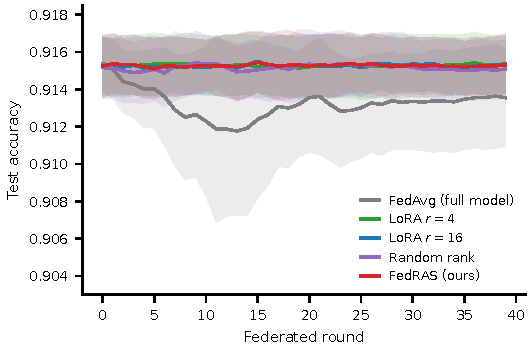
\includegraphics[width=\linewidth]{recolored_figures/fig_trainer_nominal}\\[1pt]
{\small (a) nominal deadline: accuracy}
\end{minipage}\hfill
\begin{minipage}[t]{0.49\columnwidth}
\centering
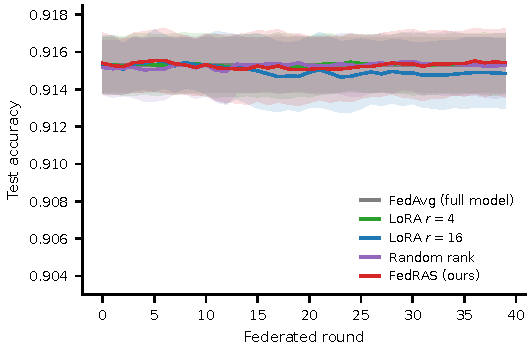
\includegraphics[width=\linewidth]{recolored_figures/fig_trainer_stress}\\[1pt]
{\small (b) 0.1\,s deadline: accuracy}
\end{minipage}\\[4pt]
\begin{minipage}[t]{0.49\columnwidth}
\centering
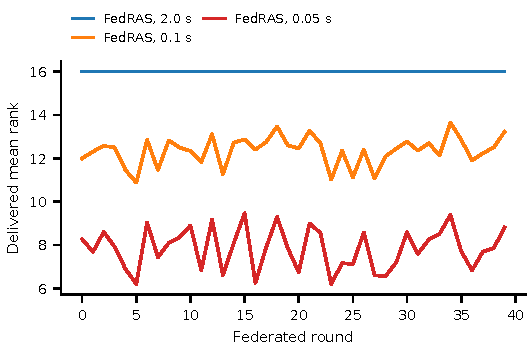
\includegraphics[width=\linewidth]{recolored_figures/fig_rank_dynamics}\\[1pt]
{\small (c) delivered rank per round}
\end{minipage}\hfill
\begin{minipage}[t]{0.49\columnwidth}
\centering
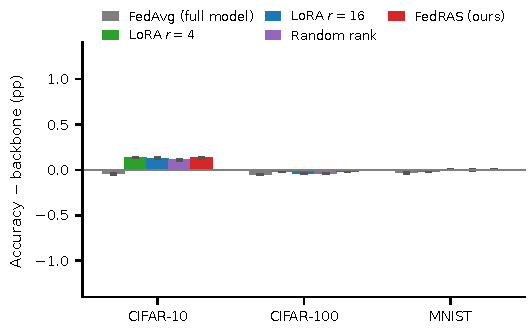
\includegraphics[width=\linewidth]{recolored_figures/fig_cross_dataset}\\[1pt]
{\small (d) accuracy across datasets}
\end{minipage}
\caption{Real-trainer experiments (CIFAR-10, means over seeds). (a)~At the nominal deadline all rank policies hold the pretrained-backbone accuracy. (b)~Under the 0.1\,s deadline all methods remain stable while full-model updates deliver nothing and stay at the backbone. (c)~FedRAS is link-aware: delivered rank holds 16, tracks 13, and tracks 8 under the 2.0, 0.1, and 0.05\,s deadlines, against the fixed annealing schedule of the SA-FedLoRA-style baseline. (d)~Final accuracy across datasets; the parity is not CIFAR-10-specific (numbers in Table~\ref{tab:trainermain}(b)).}
\label{fig:trainermain}
\end{figure}

\begin{table}[p]
\centering\scriptsize\setlength{\tabcolsep}{3pt}\renewcommand{\arraystretch}{0.9}
\caption{Real-trainer experiments (non-IID CIFAR-10 unless stated). Accuracy is round-40 test accuracy; timely delivery ratio, bytes per round (rounds 30--39, attempted uplink), and mean delivered rank follow the definitions of Section~\ref{sec:eval}. (a) Deadline ladder. (b) Extended stress matrix, five seeds. (c) External baselines, ten seeds. (d) Scheduling arms, 1.0\,MB budget. (e) Component ablations, five seeds.}
\label{tab:trainermain}
\resizebox{\columnwidth}{!}{%
\begin{tabular}{l cccc cccc cccc}
\toprule
\multicolumn{13}{l}{\emph{(a) Deadline ladder}}\\[1pt]
& \multicolumn{4}{c}{nominal 2.0\,s} & \multicolumn{4}{c}{deadline 0.1\,s} & \multicolumn{4}{c}{deadline 0.05\,s}\\
\cmidrule(lr){2-5}\cmidrule(lr){6-9}\cmidrule(lr){10-13}
Method & Acc. & Timely & MB & Rank & Acc. & Timely & MB & Rank & Acc. & Timely & MB & Rank\\
\midrule
FedAvg (full model) & $.9135\pm.0027$ & 0.17 & 52.86 & --- & $.9153\pm.0015$ & 0.00 & 52.86 & --- & $.9147\pm.0016$ & 0.00 & 52.86 & ---\\
FedLoRA $r{=}4$ & $.9154\pm.0016$ & 0.75 & 0.23 & 4.0 & $.9154\pm.0016$ & 0.62 & 0.23 & 4 & $.9144\pm.0015$ & 0.57 & 0.23 & 4\\
FedLoRA $r{=}16$ & $.9153\pm.0015$ & 0.73 & 0.90 & 16.0 & $.9149\pm.0019$ & 0.41 & 0.90 & 16 & $.9143\pm.0020$ & 0.27 & 0.90 & 16\\
Random rank & $.9151\pm.0016$ & 0.76 & 0.42 & 7.3 & $.9153\pm.0017$ & 0.56 & 0.42 & 6.2 & $.9143\pm.0015$ & 0.46 & 0.42 & 5.7\\
FedRAS (ours) & $.9153\pm.0016$ & 0.73 & 0.90 & 16.0 & $.9154\pm.0018$ & 0.49 & 0.69 & 12.7 & $.9143\pm.0014$ & 0.49 & 0.44 & 8.1\\
\bottomrule
\end{tabular}%
}\\[5pt]
\begin{tabular}{l ccccc}
\toprule
\multicolumn{6}{l}{\emph{(b) Extended stress matrix (round-40 accuracy)}}\\[1pt]
Scenario & FedAvg & $r{=}4$ & $r{=}16$ & Random & FedRAS\\
\midrule
deadline 10\,s & 0.9134 & 0.9144 & 0.9145 & 0.9141 & 0.9143\\
mobility 0.7 & 0.9115 & 0.9143 & 0.9141 & 0.9145 & 0.9141\\
$\alpha{=}0.1$ & 0.9022 & 0.9139 & 0.9107 & 0.9130 & 0.9109\\
$\alpha{=}1.0$ & 0.9142 & 0.9143 & 0.9144 & 0.9141 & 0.9144\\
CIFAR-100, 2.0\,s & 0.6925 & 0.6928 & 0.6926 & 0.6926 & 0.6929\\
CIFAR-100, 0.1\,s & 0.6927 & 0.6927 & 0.6929 & 0.6927 & 0.6928\\
MNIST, 2.0\,s & 0.9947 & 0.9949 & 0.9951 & 0.9950 & 0.9951\\
MNIST, 0.1\,s & 0.9947 & 0.9949 & 0.9950 & 0.9949 & 0.9950\\
\bottomrule
\end{tabular}\\[3pt]
\resizebox{\columnwidth}{!}{%
\begin{tabular}{l cccc cccc}
\toprule
\multicolumn{9}{l}{\emph{(c) External baselines}}\\[1pt]
& \multicolumn{4}{c}{nominal 2.0\,s} & \multicolumn{4}{c}{deadline 0.1\,s}\\
\cmidrule(lr){2-5}\cmidrule(lr){6-9}
Method & Acc. & Timely & MB & Rank & Acc. & Timely & MB & Rank\\
\midrule
SA-FedLoRA-style annealing & $.9154\pm.0016$ & 0.75 & 0.29 & 5.1 & $.9153\pm.0016$ & 0.62 & 0.29 & 5.0\\
Oort-style utility, fixed rank & $.9150\pm.0020$ & 0.76 & 0.45 & 8.0 & $.9149\pm.0019$ & 0.54 & 0.45 & 8.0\\
Joint A/B, plain averaging & $.9152\pm.0016$ & 0.73 & 0.90 & 16 & $.9148\pm.0019$ & 0.41 & 0.90 & 16\\
\bottomrule
\end{tabular}%
}\\[5pt]
\resizebox{\columnwidth}{!}{%
\begin{tabular}{l cccc cccc}
\toprule
\multicolumn{9}{l}{\emph{(d) Scheduling arms (FedLoRA $r{=}16$ reference in (a))}}\\[1pt]
& \multicolumn{4}{c}{nominal 2.0\,s, ten seeds} & \multicolumn{4}{c}{stress 0.1\,s, five seeds}\\
\cmidrule(lr){2-5}\cmidrule(lr){6-9}
Arm & Acc. & Timely & MB & Rank & Acc. & Timely & MB & Rank\\
\midrule
Full DP (grid assignment) & $.9151\pm.0016$ & 0.82 & 0.90 & 16.0 & $.9138\pm.0011$ & 0.55 & 0.87 & 15.4\\
Same-cohort DP & $.9152\pm.0019$ & 0.73 & 0.90 & 16.0 & $.9139\pm.0014$ & 0.51 & 0.70 & 12.7\\
Fair cohort (FedRAS rule) & $.9153\pm.0016$ & 0.73 & 0.90 & 16.0 & $.9144\pm.0018$ & 0.51 & 0.70 & 13.0\\
\bottomrule
\end{tabular}%
}\\[5pt]
\begin{tabular}{l cc}
\toprule
\multicolumn{3}{l}{\emph{(e) Component ablations (nominal deadline)}}\\[1pt]
Configuration & Accuracy & Min.\\
\midrule
Full system (ours) & $.9144\pm.0013$ & ---\\
w/o capacity term & $.9145\pm.0014$ & ---\\
w/o frozen $A$ (joint A/B) & $.9144\pm.0015$ & ---\\
w/o rank mask (random ranks, 0.1\,s) & $.9145\pm.0016$ & ---\\
\end{tabular}
\hfill
\begin{tabular}{l cc}
\toprule
Configuration & Accuracy & Min.\\
\midrule
w/o server momentum & $.9143\pm.0013$ & ---\\
frozen $A$, lr 0.02 & $.9130\pm.0012$ & 0.913\\
joint A/B, lr 0.02 & $.9132\pm.0012$ & 0.912\\
\bottomrule
\end{tabular}
\end{table}

\subsection{Evaluation with the federated LoRA trainer}
\label{sec:traineval}

\subsubsection{Accuracy parity and rank invariance}
Table~\ref{tab:trainermain}(a) reports ten-seed means and standard deviations after 40 federated rounds on CIFAR-10. All LoRA methods hold the backbone accuracy within one standard deviation of 0.914, whether the rank is fixed at 4, fixed at 16, drawn at random, or selected by the rank rule. Full-parameter updates spend orders of magnitude more bytes per round (Table~\ref{tab:audit}) and lose roughly three quarters of their timely deliveries because their payloads rarely fit the round deadline. The cross-dataset results in Fig.~\ref{fig:trainermain}(d) and Table~\ref{tab:trainermain}(b) repeat the parity at 0.693 on CIFAR-100 and 0.995 on MNIST. At the nominal deadline the rank rule selects rank 16 for every client of every round, so FedRAS coincides with fixed rank 16 in bytes and timeliness, and in accuracy up to floating-point nondeterminism; this identity, rather than a tuned advantage, is what the nominal regime is meant to show. Fig.~\ref{fig:trainermain}(a) shows the corresponding trajectories, stable over the 40 rounds for every rank policy.

\textbf{Delivered-update norms.} The capacity law of \eqref{eq:cap} is anchored in measured updates. The trainer logs the mean Frobenius norm of each round's delivered updates; pooled over the ten nominal seeds, the norm grows from $0.0158$ at rank 4 to $0.0297$ at rank 16, a ratio of $1.9$ against the square-root law's $2.0\times$ and linear payload growth's $4\times$, and the 0.1\,s deadline reproduces the ratio ($1.9$). The diminishing returns that \eqref{eq:cap} prices are therefore a measured property of the delivered updates, not a modeling assumption.

\subsubsection{Deadline stress}
\textbf{Delivered-rank adaptation.} Table~\ref{tab:trainermain}(a) tightens the deadline to 0.1\,s and 0.05\,s. Three effects emerge. First, FedRAS downshifts under pressure. Its delivered mean rank falls from 16.0 at the nominal deadline to 12.7 at 0.1\,s and 8.1 at 0.05\,s, where the delivery hazard \eqref{eq:hazard} makes rank-16 payloads marginal. Second, downshifting pays. At 0.1\,s, FedRAS delivers 0.49 timely updates against 0.41 for fixed rank 16 while transmitting 0.69\,MB against 0.90\,MB, i.e., 23\% fewer bytes; at 0.05\,s the gap widens to 0.49 against 0.27 timely deliveries at 51\% fewer bytes. Third, full-parameter updates collapse completely. Their timely delivery ratio is 0.00 at both stress deadlines, so not a single full-size update arrives on time in any seed; the reported stress accuracy of this row is exactly the per-seed pretrained backbone ($0.914\pm0.002$ across seeds), whose spread explains the nonzero standard deviation.

\textbf{Why downshifting dominates.} The trade is favorable because payload grows linearly in the rank while delivery probability falls convexly once the transmission time approaches the deadline. Near the deadline boundary, halving the rank roughly halves the transmission time and moves the update out of the hazard region, whereas the capacity given up is bounded by the saturating curve of $G(r)$; at a slack deadline, the same bytes buy no additional delivery probability, so holding the high rank is free. The scheduler is in effect buying delivery probability where its price is low and declining to buy it where its price is high. This is also why the delivered mean rank moves while accuracy stays at parity: in this setting the binding constraint on learning is delivery, not adaptation capacity, and the scheduler relieves the former without touching the latter.

\textbf{Against low-rank baselines.} The same stress cells place the remaining policies on one delivery--capacity trade-off. Random-rank, Oort-style, and annealed schedules deliver \emph{more} timely updates at \emph{fewer} bytes than FedRAS (0.56, 0.54, and 0.62 versus 0.49; 0.42, 0.45, and 0.29 versus 0.69\,MB; Table~\ref{tab:trainermain}(a),(c)) while holding delivered ranks of 6.2, 8.0, and 5.0 against 12.7. The evaluation therefore claims no network-side dominance over these policies. Its claim is threefold: FedRAS reaches comparable delivery behavior while preserving roughly twice the delivered adaptation capacity at equal accuracy; within the capacity-preserving regime its link-conditioned schedule strictly dominates fixed rank 16 on both network metrics; and the trade-off itself is priced from observed link state rather than followed on a fixed path. Whether the preserved capacity converts into accuracy under longer horizons or weaker backbones remains open (Section~\ref{sec:discussion}).

\textbf{Mechanism and replication.} Accuracy spreads remain within about two standard deviations, which is consistent with the parity claim. The scheduling metrics are where the methods separate. Fig.~\ref{fig:trainermain}(b) shows the ten-seed stress trajectories, and Fig.~\ref{fig:trainermain}(c) visualizes the mechanism directly: the delivered rank of FedRAS holds 16 under the nominal deadline, tracks 13 under the 0.1\,s deadline, and tracks 8 under the 0.05\,s deadline, whereas the annealed baseline follows its fixed heat--cool path regardless of link state. Under the statistical protocol of Section~\ref{sec:eval}, the ten-seed replication confirms these differences at conventional significance levels: at the 0.1\,s deadline, FedRAS transmits 23\% fewer bytes than fixed $r{=}16$ (mean paired saving, bootstrap 95\% confidence interval $[21\%,27\%]$, two-sided Wilcoxon $p{=}0.002$); it delivers a higher timely delivery ratio in ten of ten seed pairs (Wilcoxon $p{=}0.002$), by $+22\%$ as the ratio of seed means; and its accuracy is statistically equivalent within the $\pm0.5$ percentage-point margin (TOST $p<10^{-6}$).

\subsubsection{Extended stress matrix}
Table~\ref{tab:trainermain}(b) extends the study along further axes. A mobility-only scenario with Beta$(0.7,5)$ mobility at the nominal deadline leaves all LoRA policies at parity, so mobility alone does not force downshifting at this deadline. Extreme label heterogeneity with $\alpha{=}0.1$ reveals a second-order effect: rank-16 updates lose 0.32 percentage points relative to rank 4, consistent with capacity-amplified client drift, and full-parameter updates lose the most. FedRAS follows the rank-16 trajectory here, so a heterogeneity-aware downshift is a natural extension. Loosening the deadline to 10\,s restores full-model timely delivery to 0.52 without changing any LoRA accuracy. Repeating the 0.1\,s deadline on CIFAR-100 and MNIST reproduces the CIFAR-10 stress picture. The scheduling conclusions are therefore not dataset-specific; Fig.~\ref{fig:sens} shows the matching sensitivity sweeps over provisioned width, cohort size, and $\alpha$. Per-decision scheduling cost is negligible in all these settings: the per-client rank rule costs sub-millisecond per decision, orders of magnitude below the full grid-scheduling DP of Section~\ref{sec:dp_study}.

\begin{figure}[t]
\centering
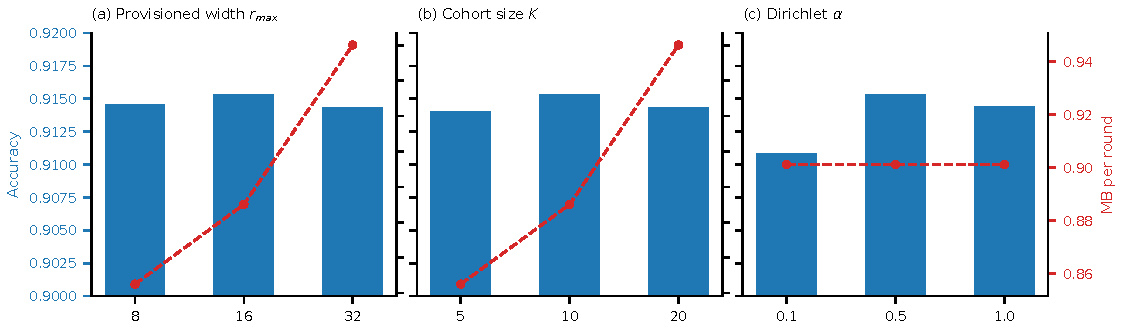
\includegraphics[width=0.98\columnwidth]{recolored_figures/fig_sensitivity}
\caption{Sensitivity of the trainer to provisioned adapter width, cohort size, and label heterogeneity on CIFAR-10 with FedRAS (five seeds per variant; the nominal reference column uses ten seeds). Accuracy is flat in $r_{\max}$ and cohort size, with a second-order drop only at $\alpha{=}0.1$; the dominant effect of all three axes is on bytes and delivered updates (red, right axis).}
\label{fig:sens}
\end{figure}

\textbf{SAGIN link profile.} Grouping the 20 clients into ground, aerial, and satellite classes with distinct rate and mobility laws reproduces the aggregate parity at the nominal deadline while exposing the expected per-class structure: timely delivery is 0.71 for ground, 0.61 for aerial, and 0.49 for satellite clients. At this deadline the scheduler holds rank 16 across all classes, so the class gap reflects the link laws alone rather than rank allocation. This profile is a parameterized link model, not a measured trace; its role is to show that the scheduler responds sensibly to client-class heterogeneity.

\subsubsection{External baselines}
\textbf{Baseline behavior.} Table~\ref{tab:trainermain}(c) reports the three external baselines of the setup in the real trainer. The link-oblivious annealing schedule settles at low rank and therefore buys timely delivery at the lowest byte cost among the baselines, but it cannot increase rank when links improve. The Oort-style selector improves selection at fixed rank. Joint A/B training matches frozen-factor training at the adopted learning rate, and the ablations find no stability separation at an elevated learning rate either, so the case for the frozen factor rests on exactness and upload reduction rather than on an observed stability gap.

\subsubsection{Scheduling variants}
\label{sec:dpvfair}
\textbf{Arms under evaluation.} To attribute the value of exact scheduling, the three arms defined in the setup are compared in the real trainer, over ten seeds at the nominal deadline and five seeds under stress. The full grid arm solves the GridDP assignment (Section~\ref{sec:gdp}) over the entire 20-client population under the participation cap and a 1.0\,MB budget, which equals ten rank-16 grid costs, so the budget binds only through downshifting or skipping. The same-cohort arm draws the identical cohort as fair cohort and restricts the same dynamic program to those candidates.

\textbf{Where exactness pays.} Table~\ref{tab:trainermain}(d) yields a clean decomposition. At the nominal deadline, the same-cohort DP coincides exactly with the per-client argmax rule, as Proposition~\ref{prop:cohort} predicts when the all-rank-16 profile fits the budget; the full DP's timely-delivery gain ($+9$ percentage points) comes entirely from admission over the wider candidate pool. Under the 0.1\,s deadline the pattern persists: the in-cohort DP matches the argmax rule, while the full DP delivers more timely updates at proportionally more bytes. Exactness therefore pays through admission control over a heterogeneous pool, not through rank allocation inside a cohort, where the cheap per-client rule is already optimal (Proposition~\ref{prop:cohort}). This delimits when full grid scheduling is worth its coordination cost.

\subsubsection{Component ablations}
\textbf{Component contributions.} Table~\ref{tab:trainermain}(e) reports component ablations at the nominal deadline. In the parity regime, no removal measurably changes final accuracy, which is consistent with the claim that accuracy is carried by the backbone and not by the scheduler. The components instead shape scheduling behavior and aggregation correctness. Removing the capacity term collapses FedRAS to the minimum rank, the degenerate delivery-only policy that the capacity term exists to prevent; its capacity cost is invisible at nominal deadlines but material in the simulator, where reliability-only optimization loses 28 points of utility against rank 16 (Table~\ref{tab:scalemain}(a)). Removing server momentum is accuracy-neutral here. The rank mask itself is network-metric-neutral at fixed rank policy: with the random-rank rule at the 0.1\,s deadline, masked and unmasked aggregation give 0.9143 and 0.9145 final accuracy with identical byte and timeliness profiles. The mask is nonetheless what keeps heterogeneous-rank aggregation per-slice exact whenever ranks mix, as Proposition~\ref{prop:agg} states, and its absence dilutes high-rank coordinates under mixed-rank rounds.

\textbf{Stability at elevated learning rate.} Under the elevated learning rate of 0.02, the frozen-factor rule and joint A/B training are statistically indistinguishable, with final accuracies of 0.9130 and 0.9132 and transient minima of 0.913 and 0.912 across rounds and seeds. The stability separation between the two aggregation rules observed in our preliminary stylized-payload experiments does not survive the corrected implementation at this horizon, so the frozen-factor rule is justified by the exactness of Proposition~\ref{prop:agg} and by its single-factor uploads, not by an empirical stability margin at this scale.

\subsection{Large-scale scheduling simulation}

\subsubsection{Scheduler behavior across operating regimes}
\label{sec:simsim}
\textbf{Regime comparison.} Table~\ref{tab:scalemain}(a) summarizes the simulator across regimes at the final round. In the nominal regime, FedRAS matches fixed rank 16 and dominates every low-rank policy. Under the 0.1\,s deadline, FedRAS leads fixed rank 16 at 21\% fewer bytes, and full-model updates deliver nothing. Under the binding 1.2\,MB budget, full-model updates cannot be admitted even once, while FedRAS and rank 16 tie. The mobility-stress and 1000-client regimes show the same pattern: FedRAS and fixed rank 16 coincide at utility 0.94 with timely delivery 0.85 (five seeds) under mobility stress, and at utility 0.92 with timely delivery 0.73 at 1000 clients, so scheduling separates only where deadlines or budgets bind. A final cell repeats the stylized protocol of the earlier literature: with the $s(r)$ payload model the ordering is preserved, confirming that the conclusions are not an artifact of the payload accounting.

\textbf{Where the simulator gain comes from.} The 0.1\,s regime makes the allocation mechanism visible. Fixed rank 16 spends uniformly, so weak-link clients consume bytes and miss deadlines while strong-link clients remain under-served; FedRAS reallocates instead, holding high ranks for clients whose delivery probability survives them and downshifting or skipping the rest --- the allocation a budget-constrained planner would make by hand. Reliability-only optimization shows the opposite failure: it buys timely delivery by collapsing clients toward the minimum rank, paying for reliability with capacity. The dynamic program sits between these extremes because the objective prices capacity and delivery in a common unit, and the grid renders the resulting knapsack exactly solvable rather than approximately.

\textbf{Trajectories.} Fig.~\ref{fig:sim} shows the nominal and 0.1\,s trajectories, and Fig.~\ref{fig:simreg} the network-side view across regimes. Across the reported regimes, FedRAS is numerically best or tied for best in the utility column of Table~\ref{tab:scalemain}(a), with the reliability-only and annealed policies retaining a timely-delivery lead bought at substantially lower delivered capacity.

\begin{table}[p]
\centering\footnotesize
\caption{Experiments at 500-client scale (five seeds unless noted). (a) Scheduler simulation across regimes; the utility column is the bounded scheduling utility of Section~\ref{sec:eval} and must not be read as dataset accuracy, MB is the attempted uplink payload of admitted clients in the final round billed on the same 0.01\,MB ceiling grid as budget admission, and FedAvg refers to full-model updates at their real serialized size. (b) Solver study with $K{=}25$ and 30 instances per cell on the identical ceiling grid; the table reports heuristic objective loss relative to the grid-based DP and DP runtime.}
\label{tab:scalemain}
\emph{(a) Scheduler simulation across regimes}\\[2pt]
\resizebox{0.98\columnwidth}{!}{%
\begin{tabular}{l ccc ccc ccc}
\toprule
& \multicolumn{3}{c}{Nominal 2.0\,s} & \multicolumn{3}{c}{Deadline 0.1\,s} & \multicolumn{3}{c}{Budget 1.2\,MB}\\
\cmidrule(lr){2-4}\cmidrule(lr){5-7}\cmidrule(lr){8-10}
Method & Util. & Timely & MB & Util. & Timely & MB & Util. & Timely & MB\\
\midrule
FedAvg (full) & .310 & .34 & 26.5 & .093 & .00 & 26.5 & .093 & .00 & 0.0\\
$r{=}4$ & .744 & .75 & 0.8 & .689 & .64 & 0.8 & .744 & .75 & 0.8\\
$r{=}16$ & .914 & .73 & 2.5 & .763 & .42 & 2.5 & .797 & .76 & 1.2\\
Random & .816 & .75 & 1.3 & .709 & .57 & 1.3 & .803 & .75 & 1.2\\
Reliability-only & .635 & .76 & 0.5 & .606 & .70 & 0.5 & .635 & .76 & 0.5\\
SA-annealing & .842 & .76 & 0.5 & .730 & .70 & 0.5 & .796 & .76 & 0.5\\
FedRAS (ours) & .914 & .73 & 2.5 & \textbf{.781} & .50 & 2.0 & \textbf{.797} & .76 & 1.2\\
\bottomrule
\end{tabular}%
}\\[6pt]
\emph{(b) Solver study}\\[2pt]
\resizebox{\columnwidth}{!}{%
\begin{tabular}{cc cccc c}
\toprule
Deadline (s) & Budget (MB) & Greedy val/byte & Greedy value & Cohort myopic & Fixed $r{=}16$ & DP time (ms)\\
\midrule
2.0  & 30  & 63.6\% & 0.0\% & 40.9\% & 0.0\% & 421\\
2.0  & 4   & 63.6\% & 0.0\% & 40.9\% & 0.0\% & 51\\
2.0  & 1.2 & 47.8\% & 28.4\% & 48.9\% & 28.4\% & 23\\
1.0  & 30  & 62.7\% & 0.0\% & 40.0\% & 0.0\% & 415\\
1.0  & 4   & 62.7\% & 0.0\% & 43.0\% & 0.0\% & 51\\
1.0  & 1.2 & 47.3\% & 29.3\% & 48.3\% & 29.3\% & 23\\
0.1  & 30  & 52.8\% & 0.0\% & 51.9\% & 0.0\% & 415\\
0.1  & 4   & 52.6\% & 0.0\% & 52.0\% & 0.0\% & 51\\
0.1  & 1.2 & 41.0\% & 36.0\% & 54.8\% & 36.0\% & 23\\
\bottomrule
\end{tabular}%
}
\end{table}

\begin{figure}[t]
\centering
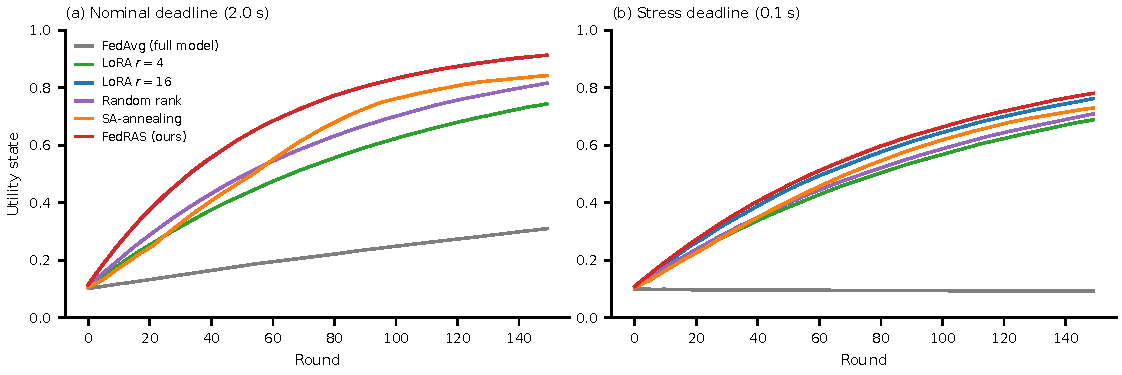
\includegraphics[width=0.98\columnwidth]{recolored_figures/fig_sim_accuracy}
\caption{Scheduler simulation utility-state trajectories (mean over five seeds). (a)~Nominal 2.0\,s deadline, where FedRAS matches fixed rank 16. (b)~0.1\,s deadline, where FedRAS downshifting separates from fixed rank 16.}
\label{fig:sim}
\end{figure}

\begin{figure}[t]
\centering
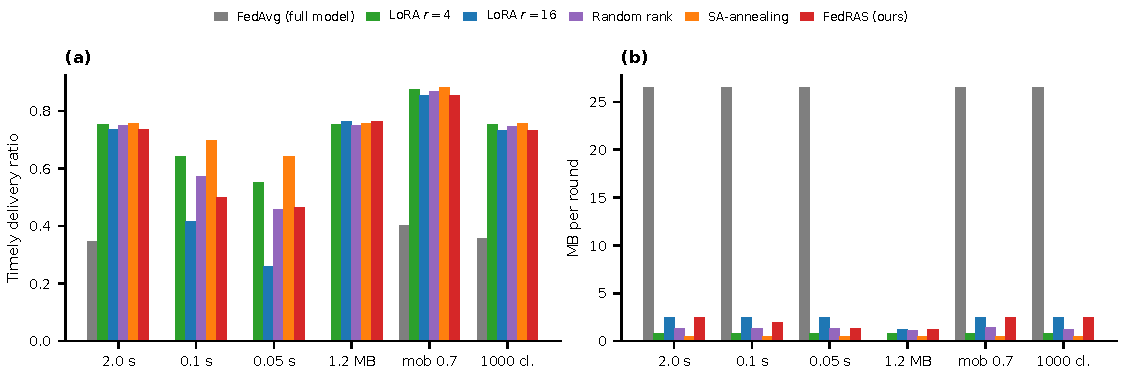
\includegraphics[width=0.98\columnwidth]{recolored_figures/fig_sim_regimes}
\caption{Timely delivery ratio and attempted bytes per method across simulator regimes (five-seed means, final round). Full-model updates deliver nothing under stress and cannot be admitted at all under the binding budget.}
\label{fig:simreg}
\end{figure}

\subsubsection{Solver optimality and runtime}
\label{sec:dp_study}
\textbf{Heuristic gaps and runtime.} Table~\ref{tab:scalemain}(b) reports the scheduling study with the identical ceiling discretization for the DP and every heuristic. When the byte budget is slack, value greedy and the fixed rank-16 rule are already optimal, so the choice of scheduler matters little; the value-per-byte greedy, by contrast, collapses to a smallest-rank preference and already loses up to 63.6\% of the objective in the slack cells. The interesting regimes are the binding ones: once the budget binds, every heuristic loses a substantial fraction of the objective --- up to 54.8\% for the cohort-myopic rule --- while the DP reaches the optimum of the discretized single-round estimated problem in every cell. Its runtime is sub-second for 500 clients across the evaluated grid widths and scales linearly to 1000 clients, as Fig.~\ref{fig:dp} shows, which is compatible with per-round scheduling at minute-scale FL rounds.

\textbf{Why the heuristics fail where they do.} Value-per-byte pricing fails structurally rather than numerically: the capacity gain $G(r)$ saturates in $r$ while payload grows linearly, so the value-per-byte ratio is maximized at the smallest rank for essentially every client and the rule degenerates to a minimum-rank schedule regardless of link state. The fixed rank-16 rule and value greedy fail only under scarcity, where the budget can no longer fund every candidate and some admissions must be forgone; choosing which candidates to drop is precisely the coupling that per-client rules cannot see. The runtime column follows the budget grid width rather than the client count: tightening the budget from 30\,MB to 1.2\,MB shrinks the discretized grid by the same ratio, which is why the DP is fastest under exactly the binding budgets that need it most.

\textbf{Grid sweep.} A dedicated grid sweep around the default step bounds the quantization error at about 3\% in the binding regime and below 1\% in slack regimes; a finer step reduces it further at a known runtime cost. The grid exactness claim of Section~\ref{sec:theory} therefore applies to a grid whose quantization error is bounded, measured, and adjustable.

\subsubsection{Delivery-predictor sensitivity}
\label{sec:calsens}
\begin{figure}[t]
\centering
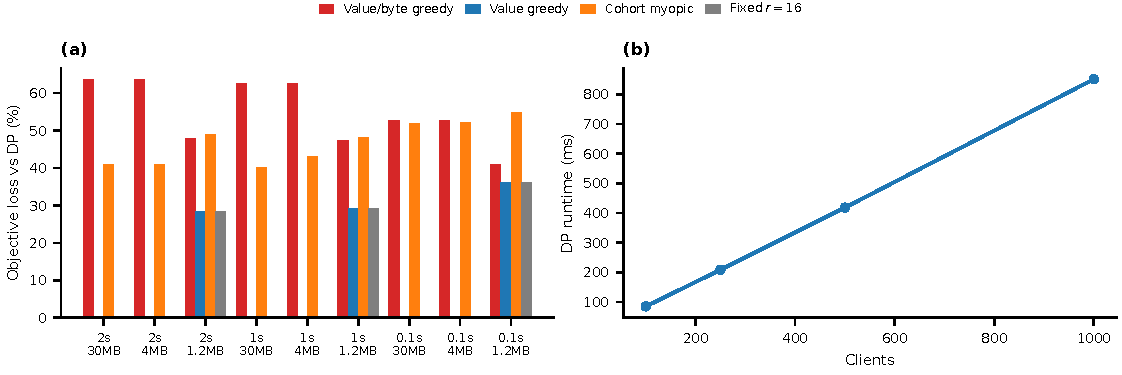
\includegraphics[width=0.8\columnwidth]{recolored_figures/fig_dp_study}
\caption{Solver study. (a)~Objective loss of the heuristics relative to the DP across deadline and budget cells. (b)~DP runtime scaling with the client population.}
\label{fig:dp}
\end{figure}

\begin{figure}[t]
\centering
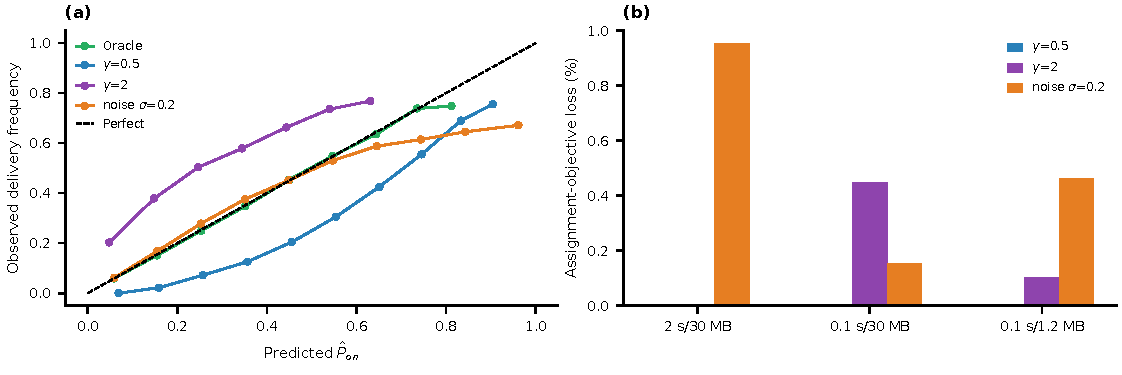
\includegraphics[width=0.8\columnwidth]{recolored_figures/fig_calibration}
\caption{Delivery-predictor calibration study (500 clients, 150 round-instances per cell). Left: reliability at the 0.1\,s deadline; with oracle link state the hazard-form predictor is calibrated by construction, while the power-distorted ($\gamma$) and noisy variants are measurably miscalibrated. Right: assignment-objective loss of optimizing against the distorted predictor, evaluated under true probabilities, at most 1\% in every cell.}
\label{fig:calib}
\end{figure}

The calibration study of Fig.~\ref{fig:calib} measures both the fidelity of the deployed predictor and the scheduling cost of its errors (500 clients). With the oracle link state of the setup, the hazard-form predictor \eqref{eq:hazard} is calibrated by construction. Deliberately distorted variants --- power distortions of the predicted probability and multiplicative lognormal noise --- are measurably miscalibrated, yet the resulting assignment-objective loss, evaluated under the true probabilities, stays below 1\% in every cell. The loss follows the structure of the error: power distortions cost most under the stress deadline, where rank ordering matters most, while noise costs most in the nominal slack cell, where it perturbs an otherwise near-uniform rank preference. Mis-prediction therefore degrades the objective smoothly rather than catastrophically, and the observed delivery outcomes of Algorithm~\ref{alg:fedras} are exactly the signal from which a per-client predictor would be recalibrated. Calibration on measured traces remains open and is taken up in Section~\ref{sec:discussion}.

\textbf{Cross-tier summary.} Taken together, the two evaluation tiers give a consistent picture. Rank choice does not measurably change accuracy for the frozen backbone at the 40-round horizon, and every accuracy comparison against fixed rank 16 passes the TOST equivalence test fixed in advance at the $\pm0.5$ percentage-point margin; an offline control that ignores delivery modeling entirely and trains on every scheduled update reaches $0.913\pm0.002$ at the nominal deadline, close to the backbone's $0.914$, separating learning capacity from delivery feasibility. The methods instead separate on the network side: FedRAS holds high ranks on healthy links and downshifts under pressure, full-parameter updates collapse once deadlines bind at real payload sizes, and the exact scheduler pays through admission over the candidate pool rather than in-cohort rank allocation (Proposition~\ref{prop:cohort}). These tests rest on ten-seed replications of the headline trainer regimes; they support the stated network-side comparisons and the accuracy equivalence, and they do not establish accuracy dominance. Section~\ref{sec:discussion} interprets these findings, states their scope conditions, and translates them into deployment guidance.

\section{Discussion and limitations}
\label{sec:discussion}
\subsection{Interpretation and deployment considerations}
\textbf{Why the gains are network-side.} The trainer demonstrates parity and equivalence, not rank-dependent accuracy gains. With a strong frozen backbone and 40 adaptation rounds, transmitted rank does not measurably change test accuracy, because the accuracy is carried by the pretrained features while the scheduler shapes which updates arrive on time and at what byte cost. Claims that low rank limits adaptation quality would require longer horizons, weaker backbones, or distribution-shifted clients.

\textbf{When FedRAS does not help.} Three settings bound the method's value. First, when the candidate pool fits within the participation cap and the budget accommodates every candidate at the provisioned width, FedRAS reduces exactly to fixed rank 16 (Proposition~\ref{prop:cohort}): the scheduling layer adds coordination cost and nothing else. FedRAS is therefore worth its coordination cost when deadlines are tight relative to real payloads or when the byte budget binds; outside those regimes, fixed rank 16 is the identical and simpler choice. Second, under extreme label heterogeneity, higher ranks lose accuracy relative to low ranks through capacity-amplified client drift, and FedRAS follows the high-rank trajectory and inherits that loss; conditioning the capacity term $G(r)$ on measured heterogeneity is left as future work. Third, under tight deadlines the weakest client class still delivers least, because downshifting protects delivery but cannot create link capacity.

\textbf{Deployment recipe.} The results translate into three planning rules for a practitioner. Calibrate the deadline ladder from the real payload of the widest provisioned rank, so that the nominal deadline leaves rank $r_{\max}$ near-constraint-free while at least one stress deadline drives its timely delivery below one half. Size the byte budget at ten times the grid cost of rank $r_{\max}$, which forces the budget to bind only through downshifting or skipping. Finally, by Proposition~\ref{prop:cohort}, use the per-client argmax rule when the pool fits within the participation cap and the budget accommodates every candidate at rank $r_{\max}$; invoke the full dynamic program whenever the pool exceeds the cap or the budget forces admissions to compete.

\textbf{Coordination cost and integration.} FedRAS is an aggregator-side module and leaves client training untouched: clients receive their assigned rank with the round schedule, slice their factors to it, and run the local objective as before. The scheduler's inputs are the estimated uplink rates, the link-state history, and the payload table of the provisioned width; its outputs are the admission and rank decisions attached to the schedule. The aggregation change is confined to the rank mask of Section~\ref{sec:aggregation}, a masked average rather than a new protocol. Its failure modes are bounded: a degraded predictor degrades the objective smoothly (Fig.~\ref{fig:calib}) rather than derailing the schedule, and if link-state estimates are unavailable altogether the scheduler falls back to fixed $r_{\max}$, which Proposition~\ref{prop:cohort} identifies as optimal whenever the pool fits the cap and the budget accommodates every candidate at that rank.

\subsection{Scope and limitations}
\textbf{Scope of claims.} The results describe network-side gains in the evaluated frozen-backbone setting; they must not be read as universal accuracy gains. The simulator capacity model is a scheduling abstraction, and its accuracy column is a bounded scheduling proxy rather than a measured dataset accuracy.

\textbf{Backbone pretraining.} The centralized pretraining stage is a documented premise inherited from parameter-efficient FL practice; the federated phase adapts but does not train the backbone. Where no server-side corpus exists, self-supervised or public-data pretraining would be needed, and the parity result should be re-verified.

\textbf{Estimator assumptions.} The hazard-form delivery model \eqref{eq:hazard} assumes the closed-form exponential realization, and the experiments supply generated link states as oracle estimates; training and processing times are included in the conceptual delivery model \eqref{eq:delivery} but are not separately measured. Production deployments should calibrate $P_{\rm on}$ per client from observed outcomes, for example with isotonic or Platt scaling monitored by a Brier score, and the scheduler treats the predictor as a plug-in. Calibration on measured wireless traces remains open.

\textbf{Myopia.} The analysis is deliberately per-round (Section~\ref{sec:theory}); a horizon-aware policy that shifts admissions across rounds as budgets carry over and mobility correlates is a natural extension.

\textbf{Evaluation horizon and topology.} The trainer conclusions are horizon-bound: forty adaptation rounds on a strong frozen backbone is precisely the regime in which rank choice is accuracy-neutral, and longer horizons, weaker backbones, or distribution-shifted clients could re-open an accuracy gap that the equivalence tests employed here cannot see. The evaluation also assumes a star topology with a trusted aggregator that collects estimated link states and computes the schedule. Nothing in the formulation requires clients to report state beyond the delivery outcomes any FL round makes observable, but a decentralized or aggregator-less variant would need a different synchronization point and is not studied here.

\textbf{Security.} The adversary and trust assumptions are stated in Section~3.4. This work proposes no protection mechanism and makes no privacy claim; differential-privacy accounting, secure aggregation, and Byzantine robustness compose orthogonally with rank scheduling \cite{bonawitz2017secureagg,wei2023pfl_dp}.

\textbf{Generality.} The trainer validates adapters on convolutional and linear layers of a CNN at $r_{\max}{=}16$ with 20 clients, and the simulator extends the population to 1000, both under synthetic link distributions. Extension to transformer backbones, measured rather than synthetic links, and larger rank sets may change the payload slope, capacity curve, and empirical conclusions. The formulation can be tested in those settings. The study does not measure energy, system overhead beyond scheduler runtime, or client fairness and therefore makes no claim about those properties.

\section{Conclusion}
\label{sec:conclusion}
This paper reframed Federated LoRA over mobile edge networks as a deadline-aware client--rank scheduling problem in which the LoRA rank is a network-visible resource accounted at its real serialized size. We derived a rank-conditioned delivery model, formulated the per-round assignment as a multiple-choice knapsack under budget and participation caps, solved the grid-discretized assignment with a pseudo-polynomial dynamic program, and stabilized heterogeneous-rank aggregation with frozen-factor rank-masked averaging in which only the trainable factor is ever transmitted.

Experiments with a real federated LoRA trainer and a 500-client scheduler simulation, with deadlines calibrated to real payloads, show that rank selection preserves backbone accuracy up to an equivalence margin fixed in advance while reshaping the network side of the exchange: under ten-seed deadline stress, FedRAS delivers 22\% more timely updates and 23\% fewer bytes than fixed rank 16 and occupies the high-capacity end of the delivery--capacity trade-off on which link-oblivious low-rank schedules sit at the opposite end, and the exact scheduler earns its cost through admission over heterogeneous candidate pools rather than through in-cohort rank allocation. The claims are conditional on the frozen-backbone setting and synthetic link models: rank scheduling adds value when deadlines bind relative to real payloads or when the byte budget binds, and reduces to fixed-rank operation otherwise. Future work includes horizon-aware stochastic scheduling, calibrated per-client delivery predictors on measured traces, protection mechanisms composed with rank scheduling, and validation on transformer backbones.

\section*{Declaration of competing interest}
The authors declare that they have no known competing financial interests or personal relationships that could have appeared to influence the work reported in this paper.

\section*{Acknowledgements}
The authors thank the members of the Information Engineering University research group for many useful discussions and for hands-on assistance with the experimental implementation.

\section*{Funding}
This research did not receive any specific grant from funding agencies in the public, commercial, or not-for-profit sectors.

\section*{CRediT authorship contribution statement}
\textbf{Wenyu Ma:} Methodology, Software, Validation, Investigation, Writing -- original draft.
\textbf{Tao Hu:} Conceptualization, Formal analysis, Supervision, Writing -- review and editing.
\textbf{Xinlei Liu:} Data curation, Investigation, Visualization.
All authors approved the submitted version and accept responsibility for the work.

\section*{Data availability}
The reproducibility package accompanying this submission contains the complete source code (trainer, simulator, solver, and analysis scripts), per-run configuration files, per-seed result tables, and the raw training logs supporting every table and figure in this study; a permanent repository DOI will be supplied at publication.

\section*{Declaration of generative AI and AI-assisted technologies in the manuscript preparation process}
During the preparation of this work the authors used AI-assisted tools for language editing and formatting support. The authors reviewed and edited all generated material and take full responsibility for the content of the published article.

\bibliographystyle{elsarticle-num}
\bibliography{references}
\end{document}
